\section{Requirements} \label{sec:Requirements}
Bennett et al. (\citeyear[][pp.~140-142]{bennett2010object}) categorises
requirements as being of three types:

\begin{description} \item[Functional Requirements]
    The system's functionality -- what it is expected to do.
    
  \item[Non-functional Requirements]
    How well the system delivers its functionality. These requirements are
    related to the performance, scalability, availability, recovery time,
    security, and others.

  \item[Usability Requirements]
    These relate to how effectively, efficiently and satisfactorily users can
    achieve their goals in the existing system. User interfaces can play a big
    part in meeting these requirements.
\end{description}

The initial iterations will be focused more on the functional and usability
requirements, paying some attention as well to specific non-functional
requirements such as performance and security.


\subsection{Functional Requirements} \label{sec:Requirements.FunctionalRequirements}
Any personal accounting system should be able to provide accurate and relevant
summaries of an individual's financial status. In order to do this, the user
needs to be able to supply the system with the necessary data so that it can be
analysed and properly converted into knowledge.

It seems fair to infer that nowadays most of a user's financial transactions
currently happen in ways that can be listed electronically (usually via their
bank or credit card statements) -- a study by Payments UK
(\citeyear{paymentsUK2017summary}), for example, indicates that there has been
a rise in debit card payments over the past few years, and that the volumes of
this type of transaction is likely to be higher than that of cash payments by
the year 2021. Therefore, an assumption has been made that the users will
require means of uploading a list of their financial transactions into the
system, and this has been identified as a functional requirement.

The system created for this project intends to do just this. Its main feature,
however, will be a feature to allow the user to categorise expenditure based on
patterns in the entries' description. However, in order not to restrict the
system to the uploading of transactions via bank or credit card statements
only, it must also be possible for a user to create entries manually.

There must also be a feature to allow the user to view summaries of the income
and expenditure over a period of time, as well as one to forecast budgets for
future periods of time based on the analysed ``financial behaviour''.

\subsubsection{Requirements Model} \label{sec:Requirements.RequirementsModel}

Use case diagrams are UML constructs which were developed by Jacobson et al.
(1992, cited \cite[][p.~154]{bennett2010object}). The use case diagram below is
used to illustrate the functional requirements listed in
\ref{sec:Requirements.FunctionalRequirements}:

\begin{figure}[ht!]
  \begin{center}
    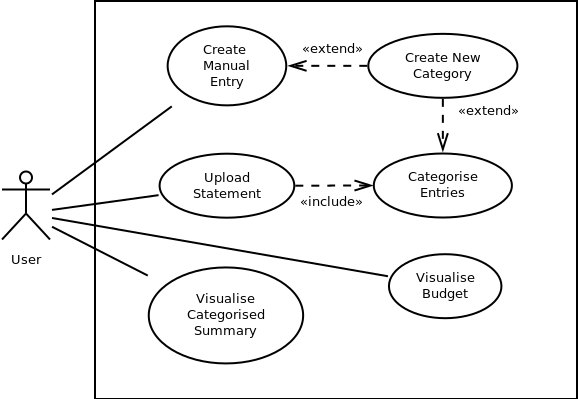
\includegraphics[width=14cm]{./contents/img/Use_Case_Diagram.png}
  \end{center}
\end{figure}
\FloatBarrier

The wireframe below was created to better illustrate the \emph{Manual Entry} requirement:
\begin{figure}[ht!]
  \begin{center}
    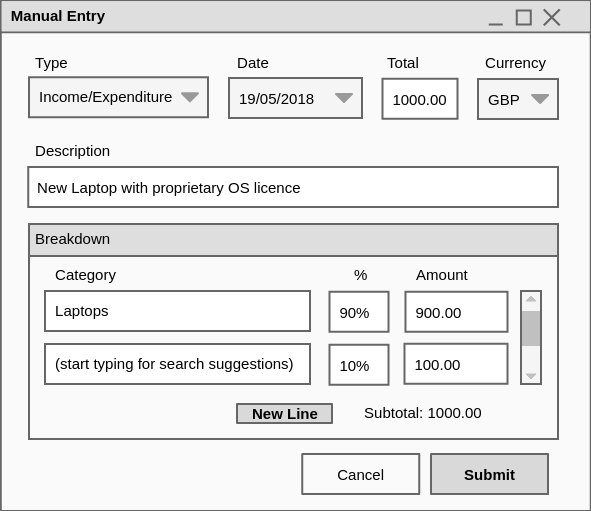
\includegraphics[width=14cm]{./contents/img/Wireframe_-_Manual_Entry.png}
  \end{center}
\end{figure}
\FloatBarrier

Also, in order to better understand the relationship between \emph{Upload
Statement} and \emph{Categorise Entries}, the activity diagram below was
developed:
\begin{figure}[ht!]
  \begin{center}
    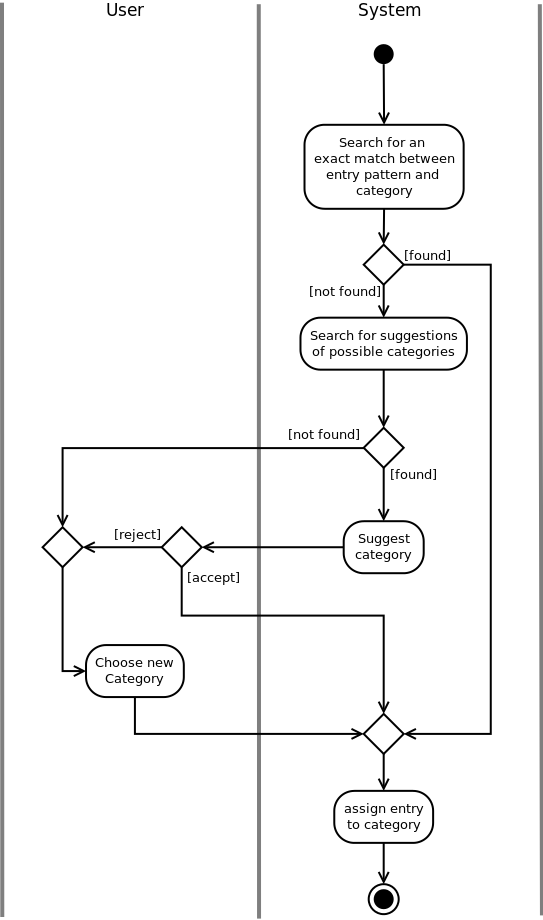
\includegraphics[width=11cm]{./contents/img/Activity_Diagram_-_Categorise_Entries.png}
  \end{center}
\end{figure}
\FloatBarrier


\subsection{Non-Functional Requirements} \label{sec:Requirements.NonFunctionalRequirements}
Use cases and use case diagrams are an appropriate tool to document functional
requirements, but not non-functional ones (Jacobson et al., 1999,
\cite[cited][p.~153]{bennett2010object}). Therefore, a separate list has been
kept in order to document the non-functional requirements, where they exist.
